% !TeX root = RJwrapper.tex
\title{Working with Daily Climate Model Output Data in R and the
\pkg{futureheatwaves} Package}
\author{by G. Brooke Anderson, Colin Eason, Elizabeth A. Barnes}

\maketitle

\abstract{%
Research on climate change impacts can require extensive processing of
climate model output, especially when using ensemble techniques to
incorporate output from multiple climate models and multiple simulations
of each model. This processing can be particularly extensive when
identifying and characterizing multi-day extreme events like heat waves
and frost day spells, as these must be processed from model output with
daily time steps. Further, climate model output is in a format and
follows standards that may be unfamiliar to most R users. Here, we
provide an overview of working with daily climate model output data in
R. We then present the \CRANpkg{futureheatwaves} package, which we
developed to ease the process of identifying, characterizing, and
exploring multi-day extreme events in climate model output. This package
can input a directory of climate model output files, identify all
extreme events using customizable event definitions, and summarize the
output using user-specified functions.
}

\section{Introduction}\label{introduction}

Research on climate change impacts can require extensive processing of
climate model output data. This is not only because output files for a
single climate model can be large, but also because of the rising
popularity of ensemble techniques \citep{IPCCch1} in which, to better
characterize uncertainty in projections, impacts are assessed for
multiple climate models, multiple simulations of each climate model, and
multiple climate experiments. Such ensemble techniques help characterize
uncertainty in projections of regional climate change over the next
century due to three distinct sources: (1) internal climate variability,
i.e.~climate noise, (2) climate model uncertainty, i.e.~the same forcing
can produce a different response in different models and (3) scenario
uncertainty, i.e.~uncertainty in future climate forcings (e.g.
\citet{hawkins2009potential}).

A key source of data for ensemble techniques is the Coupled Model
Intercomparison Project, phase 5 (CMIP5; \citet{taylor2012overview}).
This project brought together major climate modeling groups around the
world to simulate the same future radiative forcing scenarios, but with
their own models. This created an ensemble of state-of-the-art climate
model projections that allow researchers to study projections and their
uncertainties. Most of these modeling groups additionally performed more
than one simulation for each scenario and model (i.e.~multiple ensemble
members), perturbing the initial conditions by a very tiny amount to
quantify uncertainties due to internal climate variability.

We begin this article with an overview of CMIP5 climate model output
data for R users, focusing on output with a daily time step. We outline
where data from CMIP5 can be obtained as well as how to work with the
file format (netCDF) from R. We overview some R packages that can be
useful when working with this data, as well as aspects of the data
(e.g., non-standard calendars) of which users should be aware when
working with daily climate model output in R.

After this overview, we present the \CRANpkg{futureheatwaves} package,
which we created to aid in identifying and characterizing any type of
multi-day extreme event from daily climate model output (Table
\ref{tab:goals}). The impacts of multi-day extreme events must be
assessed using output in daily time step, unlike other climate impacts
that can be assessed using climate model output at monthly, seasonal, or
yearly time steps. Further, extreme events are identified based on
conditions that are rare for a certain location (e.g., 98th percentile
of local temperature distribution for identifying heat waves)
\citep{IPCCch1}. In this case, the event definition must be determined
at each study location from climate model output before events can be
identified. Finally, it is often of interest to create summaries of
multiple characteristics of these extreme events. For example, one may
be interested in determining whether the frequency or characteristics
(e.g., length, intensity) of heat waves or warm spells will change under
certain climate change scenarios \citep{IPCCch1}.

The \pkg{futureheatwaves} package handles these challenges and can be
used to identify and characterize a variety of multi-day extreme events
across different ensemble members of one or more climate models. It also
provides some functionality particularly useful in identifying and
characterizing heat waves specifically. Quantification of the impacts of
heat waves on human health suffer from additional sources of uncertainty
beyond those inherent in projections of regional changes in surface
temperature. These include: (1) uncertainty in the definition of a heat
wave itself and (2) uncertainty in the ability of communities to adapt
to changing temperatures (the adaptation scenario). This package
therefore allows the user to create and use a custom extreme event
definition to identify events in the climate model output, as well as
provides options to explore different scenarios of adaptation to heat.

\begin{table}[t]
\begin{center}
\newcolumntype{L}[1]{>{\raggedright\arraybackslash}p{#1}}
\begin{tabular}{lL{\dimexpr0.8\textwidth-2\tabcolsep\relax}}
\toprule
 & Design goals of the \pkg{futureheatwaves} package \\
\midrule
1 & Make processing of large ensembles of climate simulations more practical for researchers exploring the potential impacts of heat waves and other multi-day extreme events.\\
2 & Speed up processing time by incorporating C++ in event identification.\\
3 & Keep track of the names of climate models and number of ensemble members processed for each.\\
4 & Not only identify, but also characterize, all extreme events within each climate simulation, to allow the exploration of patterns in these characteristics across different simulations and also to allow the use of more complex impacts models, including models that incorporate event characteristics (e.g., event length, event intensity). For example, this package allows the user to apply a health effects model where risk of mortality is not the same for every heat wave, but rather is modified by heat wave length, intensity, or other measured characteristics.\\
5 & Give users extensive power in customizing the process, including allowing custom extreme event definitions.\\
6 & Allow users to easily explore the extreme events identified within all climate simulations.\\
7 & Create output that is in a ``tidy" data format, allowing it to work well with \CRANpkg{ggplot2} for visualization.\\
\bottomrule
\end{tabular}
\end{center}
\caption{Design goals for the \pkg{futureheatwaves} package.}
\label{tab:goals}
\end{table}

\section{An overview of climate model output for R
users}\label{an-overview-of-climate-model-output-for-r-users}

\subsection{CMIP5 climate model output
data}\label{cmip5-climate-model-output-data}

For climate impact studies, a main source of data is the Coupled Model
Intercomparison Project, which is currently in its fifth phase (CMIP5).
Over 20 climate modeling groups created one or more climate models
which, for this project, were run using standardized scenarios
\citep{taylor2012overview}. The resulting output is uniform across
modeling groups and has a consistent structure, which allows comparison
of simulations from different models \citep{IPCCch9}. CMIP5 climate
model output is archived at a number of different time steps (e.g.,
daily, monthly, seasonal, yearly) \citep{taylor2010cmip5}, and some
variables are reported at multiple levels in the ocean or atmosphere
(e.g., ocean temperature is reported at different ocean depths). Here,
we will focus on data with a daily time step for variables reported at a
single level (e.g., near-surface air temperature).

Each modeling group ran simulations for CMIP5 under several experiments,
with experiments varying in terms of radiative forcing scenarios through
the use of different scenarios of time-varying model inputs (greenhouse
gas emissions or concentrations, land use changes, etc.)
\citep{taylor2012overview, IPCCch9}. Experiments include historical
experiments (run using radiative forcing consistent with observed and
reconstructed data for 1850--2005), pre-Industrial control experiments,
and experiments of future scenarios of radiative forcing over the 21st
century or longer (e.g., RCP4.5, RCP8.5) \citep{taylor2012overview}.
Some modeling groups created ensembles of output for a specific model
and experiment, in which they ran the experiment multiple times with the
model with very small changes to the initial conditions.

The CMIP5 climate model output data are distributed across data nodes at
different climate modeling centers \citep{taylor2012overview}, but can
be accessed centrally at the World Climate Research Programme CMIP5 data
portal at \url{https://pcmdi.llnl.gov/search/cmip5/}. Users must
register before downloading data, and some data are restricted to
non-commercial use. There is a separate file for each combination of
climate model, experiment, modeling realm (e.g., atmosphere, ocean),
variable, time step, and ensemble member
\citep{taylor2012overview, taylor2010cmip5}. For finer time scales, the
output is further split across multiple files for specific year ranges
(e.g., 5 years of output for each file) \citep{taylor2010cmip5}. Each
file's name includes the output variable, climate model, experiment, and
ensemble member for the simulation \citep{taylor2010cmip5}.

CMIP5 files can be searched and downloaded through a point-and-click web
interface. They can also be downloaded in bulk to computers with Unix or
Mac operating systems using the \code{wget} file downloading utility.
Appropriate \code{wget} scripts can be created either through the World
Climate Research Programme CMIP5 data portal or through Earth System
Grid Federation's Search RESTful API. Tips on efficiently searching and
downloading the data, including through use of wget scripts and the
search API, are available as user tutorials through the website of the
University of Colorado Boulder's Earth System CoG (e.g.,
\url{https://www.earthsystemcog.org/projects/cog/doc/wget} for a
tutorial on downloading files using wget).

CMIP5 files are saved in Network Common Data Format (netCDF), a binary
file format that allows storage of data representing a regular array.
For climate model output at a single level (e.g., near-surface air
temperature), the data is a 3-dimensional array, with dimensions
representing time and two coordinates of location (e.g., latitude and
longitude). Figure \ref{fig:netcdfexample} provides a sketch of the
structure of netCDF files for single-level climate model output.

Each data point in the netCDF array gives the modeled value of the
variable (e.g., surface temperature) for a single time point and
location. Global climate models generate output at regularly-spaced time
steps, typically at regularly-spaced grid points around the world. The
latitude and longitude spacing of grid points vary by climate model, but
are typically 1--2 degrees for atmospheric variables in CMIP5 models
\citep{IPCCch9}. For CMIP5 climate model output, the location units are
in degrees east and degrees north for longitude and latitude,
respectively. For daily output files, the time unit is in days since a
specified origin date-time (e.g., days since 1850-01-01 00:00:00)
\citep{taylor2010cmip5}.

All CMIP5 output files are required to include certain metadata (or
``attributes'') \citep{taylor2010cmip5}, including the experiment,
forcing agents input to the model to create the simulation, time step,
institution and institutional contact information, climate model, and
modeling realm \citep{taylor2010cmip5}. The metadata also must include
units for all of the dimension variables (e.g., longitude, latitude,
time). The netCDF format allows you to access metadata and variables
describing the dimensions of the data without reading the full file into
memory.

\begin{figure}
\begin{center}
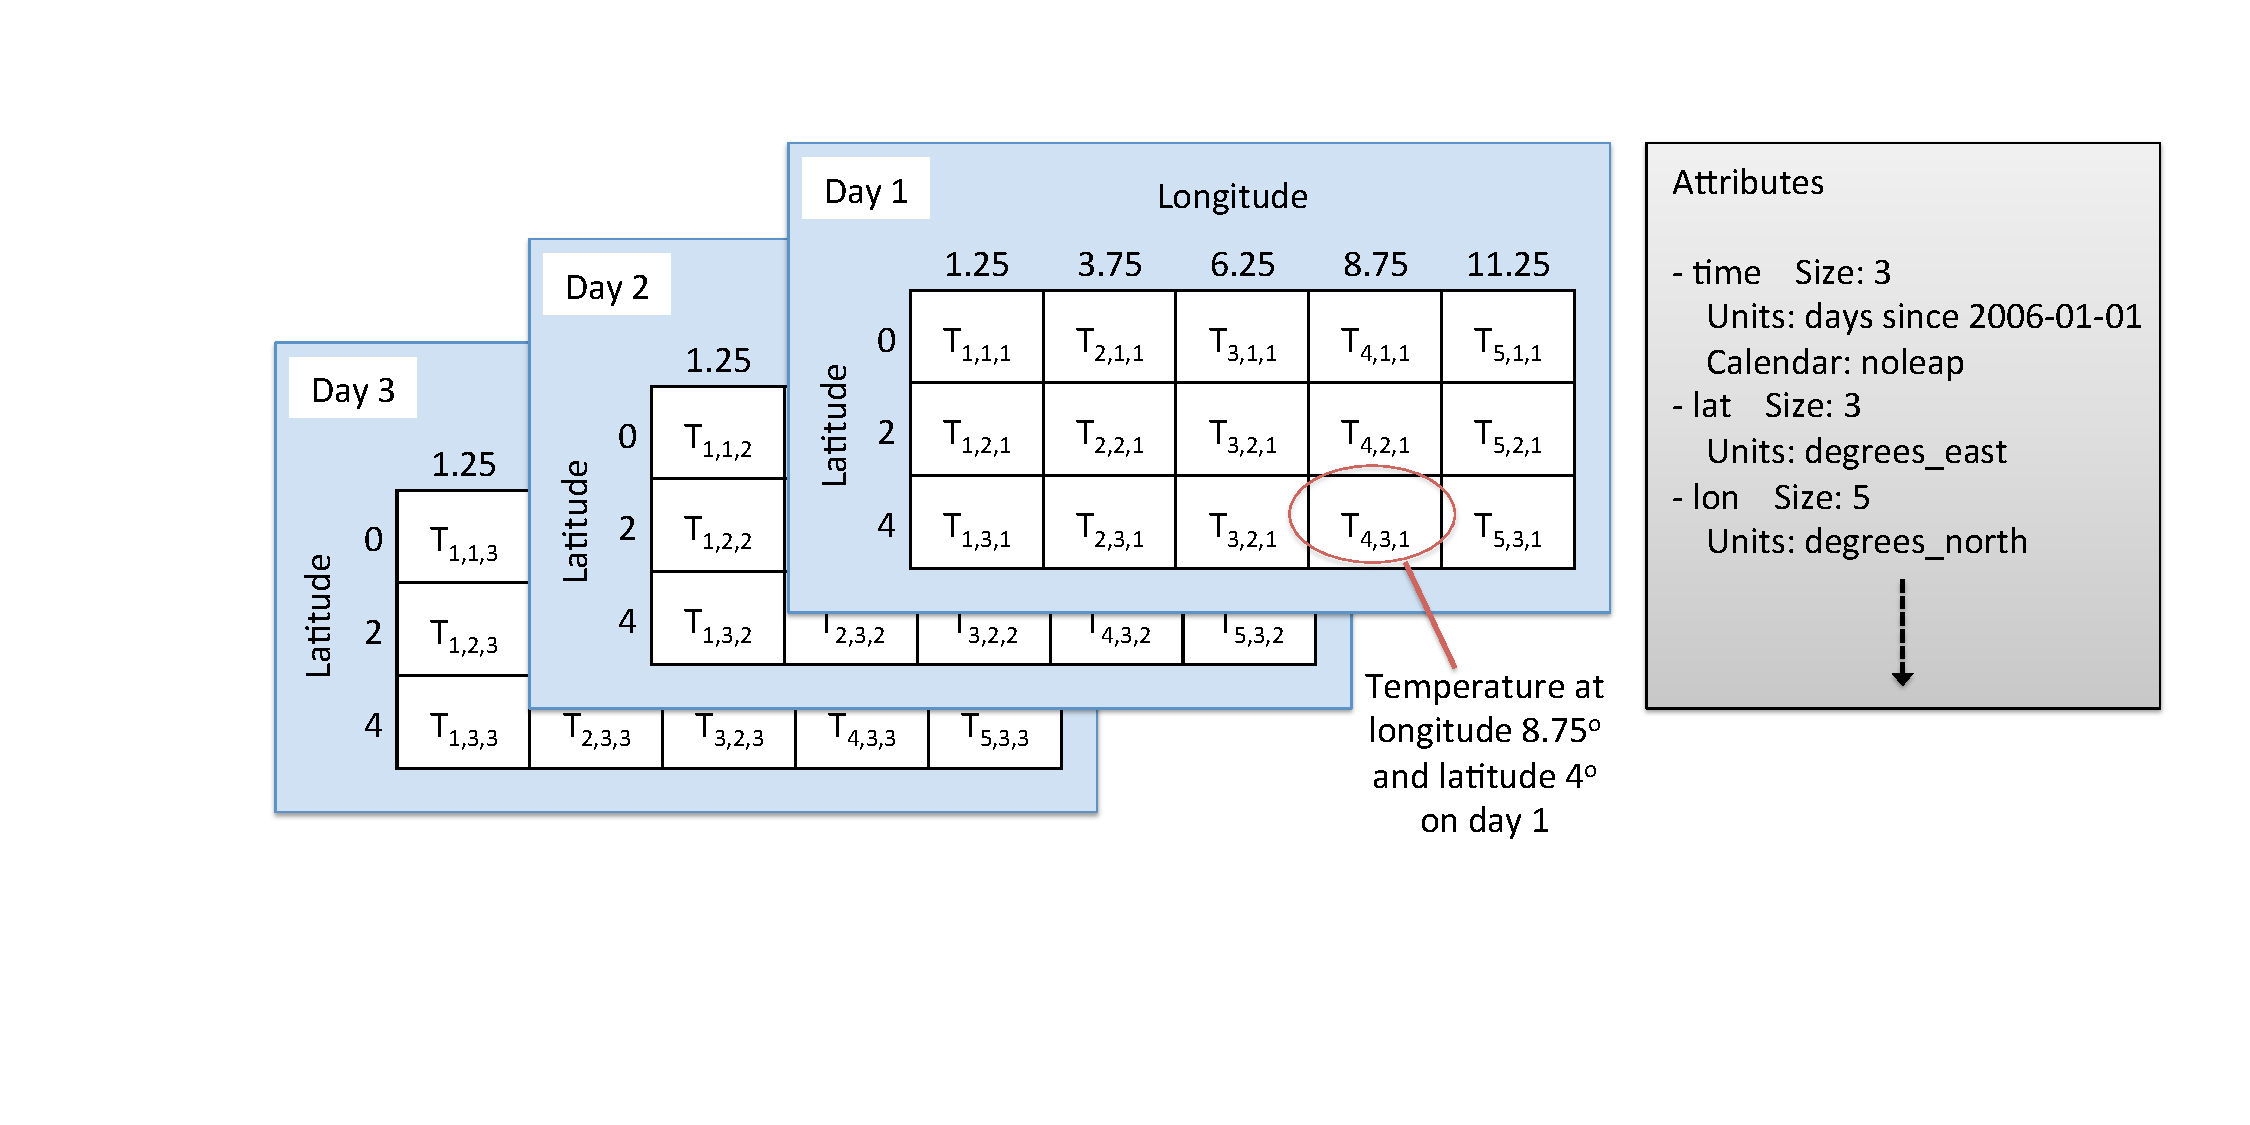
\includegraphics[width = \textwidth]{netcdf_figure}
\end{center}
\caption{Example of structure of a netCDF climate model output file for a variable reported at a single level, like near-surface air temperature. Data are stored in a three-dimensional array, with measurements at each time step and climate grid location. These data are typically indexed in the netCDF file by longitude, latitude, and time, in that order. For example, if the near-surface air temperature in the example netCDF shown here is read into an R object called \code{tas}, you can access the value for the first day at the fourth longitude and third latitude with \code{tas[4, 3, 1]}. In addition to the output variable (temperature in this example), vectors with the ordered values of each dimension (longitude, latitude, and time) can also be read in from the netCDF file, as well as attribute data (e.g., units for variables, the calendar used for time).}
\label{fig:netcdfexample}
\end{figure}

To find out more about the CMIP climate model output data,
\citet{taylor2012overview} and \citet{meehl2007wcrp} are excellent
resources.

\subsection{Working with climate model output in
R}\label{working-with-climate-model-output-in-r}

When working with daily climate model output data, challenges to R users
include: (1) the file format; (2) use of non-Gregorian calendars; and
(3) large file sizes. This section explains these challenges and offers
some strategies for dealing with them.

CMIP5 data are available in the netCDF file format. Free specialty
software exists to work with climate model output files in this format,
including a collection of command line tools developed by the Max Planck
Institute called Climate Model Operators (CDO)
\citep{schulzweida2006cdo} and an interpreted language developed by the
National Center for Atmospheric Research (NCAR) called the NCAR Command
Language (NCL) \citep{ncl}. Although such software can be used to
quickly process netCDF climate model output files, they require learning
a new language syntax, and so for R users may not be worth the
computational speed gain compared to alternative solutions that can be
scripted in the R language. While base R import functions do not exist
for netCDF files, there are a few R package extensions that allow R
users to work with the netCDF file format used for CMIP5 files directly
from R. Older packages include \pkg{ncdf} and \pkg{ncvar}, but these do
not work with the newer netCDF version 4 released in 2008 and are no
longer available through CRAN. More recent packages, including
\CRANpkg{ncdf4} \citep{CRANncdf4} and \pkg{CRANRNetCDF}
\citep{michna2013rnetcdf, RNetCDF}, work with both version 4 and
netCDF's older version 3. While climate model output data for CMIP5 are
required to conform with the earlier version (version 3)
\citep{taylor2010cmip5}, it is safer to write code using functions that
can be used with either version, in case future phases of CMIP do not
require files to conform with netCDF version 3.

You can do a number of things with netCDF files in R using these
packages. For example, \pkg{ncdf4}'s \code{nc\_open} function can be
used to open a connection to a netCDF file, and the object returned by
the function includes the file's attribute data. Once a file connection
is open, variables can be read in using the \code{ncvar\_get} function.
For example, the variables defining the dimensions of the sketched
netCDF file in Figure \ref{fig:netcdfexample} could be read into R with
\code{ncvar\_get} with the \code{varid} parameter set to ``lat'',
``lon'', or ``time''.

The climate output variable (e.g., near-surface air temperature) can
similarly be read in using \code{ncvar\_get}. In this case, the
\code{varid} parameter should be set using the appropriate CMIP5
variable name (e.g., ``tas'' for near-surface air temperature); these
variable names can be found in the CMIP Requested Output tables
\citep{taylor2010cmip5}. If only a subset of the full file is needed,
the dimensional time and location data can be used to identify the
location of the needed data in the netCDF array and this information can
then be used to read a portion of data into memory (for example, with
the \code{nc.get.var.subset.by.axes} function in
\CRANpkg{ncdf4.helpers}). Once the user is done reading in data from the
file, the connection to the netCDF should be closed (e.g., with the
\code{nc\_close} function from \pkg{ncdf4}).

\begin{figure}
\begin{center}
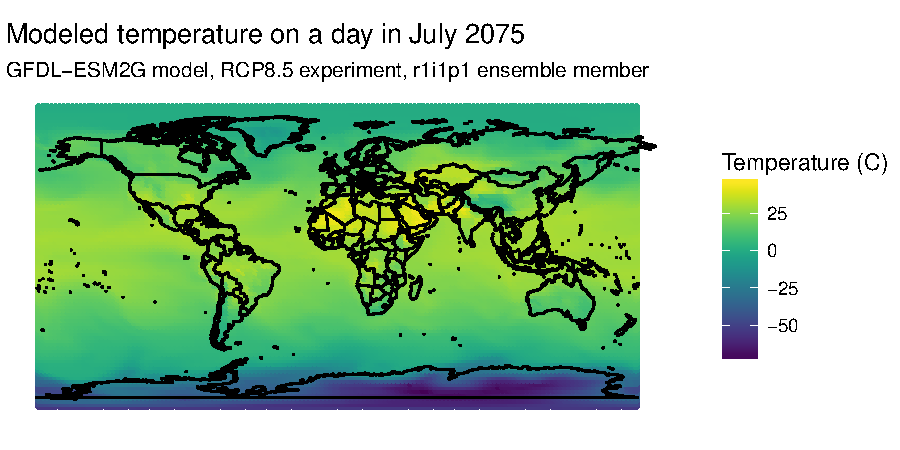
\includegraphics[width = \textwidth]{worldmapexample}
\end{center}
\caption{Example of mapping near-surface air temperature data worldwide for a single day of climate model output data. This map uses data from the Geophysical Fluid Dynamics Laboratory's Earth System Model 2G, r1i1p1 ensemble member, on a single day in the summer of 2075. Full code for recreating the map is available in the "starting\_from\_netcdf" vignette of the \pkg{futureheatwaves} package.}
\label{fig:worldmap}
\end{figure}

\begin{figure}
\begin{center}
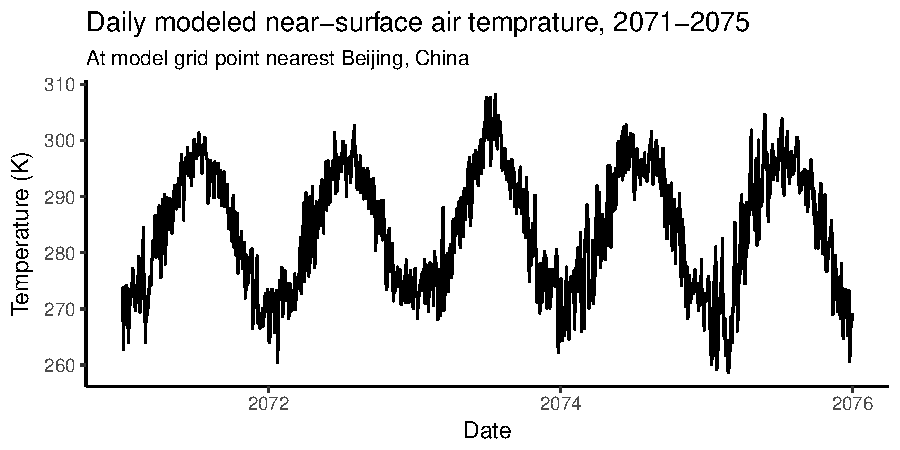
\includegraphics[width = 0.8\textwidth]{timeseriesexample}
\end{center}
\caption{Example of plotting a time series of temperature simulations between 2071 and 2075 from CMIP5 daily climate model output data for the model grid cell point closest to Beijing, China. This plot uses data from the Geophysical Fluid Dynamics Laboratory's Earth System Model 2G, r1i1p1 ensemble member. Full code for recreating the map is available in the "starting\_from\_netcdf" vignette of the \pkg{futureheatwaves} package.}
\label{fig:timeseries}
\end{figure}

A second challenge when working with climate model output data in R is
that some climate models output to non-Gregorian calendars. Since the
late 1500s, Western dates have been set using the Gregorian calendar,
which has 365.2425-day years. Some climate models, however, are run
using different calendars, including the Julian calendar (365.25-day
years), a calendar where there are no leap years (365-day years), a
calendar where every year is a leap year (366-day years), and a calendar
of twelve 30-day months (360-day years) \citep{cfconventions}. With
these non-Gregorian calendars, R's base functions for converting a
vector to a Date class based on the number of days since an origin date
(\code{as.Date}, \code{as.POSIXct}) do not return the desired values.

Two R packages provide help with non-Gregorian calendars:
\CRANpkg{PCICt} \citep{PCICt} and \CRANpkg{ncdf4.helpers}
\citep{ncdf4.helpers}. The \code{nc.get.time.series} function in
\pkg{ncdf4.helpers} pulls and uses metadata on the calendar stored in
the CMIP5 netCDF file's attributes to convert the ``time'' variable in
the file to an object of the \code{PCICt} class. This class is defined
in the \pkg{PCICt} package and provides date-like functionality for 360-
and 365-day calendars \citep{PCICt}. However, while these functions will
help with handling most CMIP5 files, the CMIP5 standards allows use of
other calendars which may not be successfully handled by these
functions, so it is important to assess whether the time variable range
in the \code{PCICt} object correctly matches the expected date ranges
for a file when processing CMIP5 data in R. While most CMIP5 climate
models use the same calendar for all experiments, a few do not; a full
table of the calendars used for each climate model and experiment,
pulled from netCDF metadata, is available at
\url{https://www.earthsystemcog.org/projects/cog/faq_data}.

Finally, the size of CMIP5 files can make them difficult to work with in
R. CMIP5 climate model output files can be as large as several
gigabytes. The size of the files can therefore be large enough that it
may make more sense to work with smaller chunks of the data in R, rather
than reading all data into memory and working with the data all at once
\citep{RCMIP5}. This problem aggregates when working with multiple
climate models and more than one ensemble member for each of those
climate models.

In addition to these general packages for working with netCDF files,
there are several R packages specifically for working with climate model
output data, including \CRANpkg{RCMIP5} \citep{RCMIP5} and \CRANpkg{wux}
\citep{wux}. However, these packages are more useful for working with
data output at time steps of a month or higher and have limited utility
with the daily climate model output data required for studies of
multi-day extreme events.

The \pkg{RCMIP5} package includes functions to read in CMIP5 data from
netCDF files, scan a directory of CMIP5 files and determine models with
continuous available data, create objects of a special \code{cmip5data}
class to work with CMIP5 data within R, and parse the file names for all
files in a directory to extract information within the file name. For
this package, most functions only work with monthly or less frequent
data \citep{RCMIP5}. While the \code{loadCMIP5} function does
successfully load daily data as a \code{cmip5data} object, most of the
methods for this object type do not do anything meaningful for daily
data. The package's \code{getFileInfo} function, however, will work with
CMIP5 files of any time step; this function identifies all CMIP5 files
in a directory and creates a data frame with information parsed from the
file name. The \code{get.split.filename.cmip5} function in the
\pkg{ncdf4.helper} package similarly can be used to parse information
contained in CMIP5 file names \citep{ncdf4.helpers}.

The \pkg{wux} package \citep{wux} includes functions that allow the user
to download CMIP5 output at a monthly time step directly from R with the
\code{CMIP5fromESGF} function. The package then uses the
\code{models2wux} function to read climate model output netCDF files and
convert it to ``WUX'' data frames, which can be used by other functions
in the package. While this function can input climate model output with
daily time steps (the ``what.timesteps'' element of the
\code{modelinput} list input must be set to ``daily''), the function
aggregates this data to a monthly or less frequent (e.g., seasonal)
aggregation when creating the WUX data frame. Therefore, while this
package provides very useful functionality for working with averaged
output of daily climate model output data or with output data at a
larger time step, it cannot easily be used to identify and characterize
multi-day extreme events like heat waves.

The functions and packages described in this section can be used with
CMIP5 netCDF files to do things in R like map near-surface air
temperatures from a single climate model on a specific day (Figure
\ref{fig:worldmap}) or pull a time series of daily near-surface air
temperature simulations at a specific climate model grid point (Figure
\ref{fig:timeseries}). The \pkg{futureheatwaves}' ``Starting from netCDF
files'' vignette
(\url{https://cran.r-project.org/web/packages/futureheatwaves/vignettes/starting_from_netcdf.html})
provides all code required to create these figures, as well as more
details and code examples on working with CMIP5 netCDF files in R.

\section{\texorpdfstring{The \pkg{futureheatwaves}
package}{The  package}}\label{the-package}

\subsection{Motivation}\label{motivation}

We created the \pkg{futureheatwaves} package to aid in identifying,
characterizing, and exploring multi-day extreme events in daily climate
model output data. While most of the discrete tasks involved in
identifying and characterizing multi-day extreme events are fairly
straightforward, the full process can be code-intensive, especially for
multi-city studies and studies that test sensitivity to how an event is
defined or that incorporate different scenarios of adaptation in the
case of events defined using a threshold relative to community climate.
Our aim in developing this package was therefore to make the full
process of identifying and characterizing these extreme events much more
convenient and so facilitate the use of multi-model, multi-ensemble
member analyses in climate impact studies conducted by non-climate
scientists.

\subsection{How the package works}\label{how-the-package-works}

\begin{widefigure}
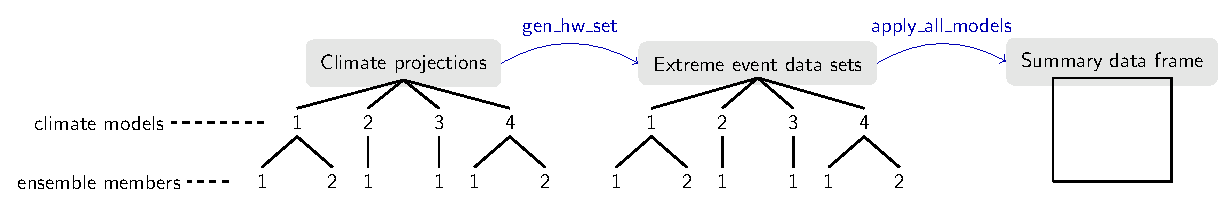
\includegraphics[width = 0.9\textwidth]{OverviewFigure}
\caption{Overview of the functionality of the \pkg{futureheatwaves} package. The package takes a directory with climate projection files (left), for one or more climate models, with one or more ensemble members for each climate model (this example figure shows four climate models with one or two ensemble members each). The \code{gen\_hw\_set} function processes these files to create a data frame for each ensemble member, identifying and characterizing all multi-day extreme events (e.g., heat waves) in the time series projection for that ensemble member. The \code{apply\_all\_models} function allows users to explore these extreme events by applying user-created functions across all the extreme event data frames, creating a summary data frame with results.}
\label{fig:overview}
\end{widefigure}

Figure \ref{fig:overview} gives an overview of the two primary functions
of the \pkg{futureheatwaves} package. First, the \code{gen\_hw\_set}
function processes a directory of climate projection files that are
stored locally on the user's computer (Figure \ref{fig:overview},
``Climate projections''), to generate a list of all extreme events in
each projection, as well as over a dozen characteristics of each
identified extreme event (Table \ref{tab:hwcharacteristics}). This
package start from files rather than R objects to avoid loading data
from all climate model ensembles at once; instead, the function loads,
processes, and saves output for a single climate model ensemble member
at a time. The extreme events are identified and characterized at one or
more study locations (e.g., cities), which the user specifies in an
input file. The extreme events identified for each ensemble member are
output as separate files in a directory specified by the user (Figure
\ref{fig:overview}, ``Extreme events datasets``).

Once the user creates these data frames of location-specific extreme
events, the \code{apply\_all\_models} function can be used to apply
custom functions across all the extreme event data frames. This
functionality allows users to create summaries of extreme events across
all climate models and ensemble members (Figure \ref{fig:overview},
right). The function can be used to generate summary statistics (e.g.,
determine average heat wave length or total frost days) or to apply more
complex functions (e.g., apply epidemiologic effect estimates across the
heat waves to generate health impact estimates).

When using this package, CMIP5 climate model output data require some
pre-processing. Data will need to be saved in a specific format, with
files stored in a specific directory structure. Full details of the
required file and directory structure are provided in the package's main
vignette
(\url{https://cran.r-project.org/web/packages/futureheatwaves/vignettes/futureheatwaves.html}),
while tips and an R script for conducting this processing starting from
CMIP5 netCDF files are given in the ``Starting from netCDF files''
vignette
(\url{https://cran.r-project.org/web/packages/futureheatwaves/vignettes/starting_from_netcdf.html}).

This package can be used for study locations worldwide. The ``Starting
from netCDF files'' package vignette provides an example of using this
package to identify and explore future heat waves in several Chinese
cities.

\begin{table}
\newcolumntype{L}[1]{>{\raggedright\arraybackslash}p{#1}}
\begin{tabular}{lL{\dimexpr0.8\textwidth-2\tabcolsep\relax}}
\toprule
Column name & Description of characteristic \\
\midrule
\code{mean.var} & Average daily value of the variable across all days in the extreme event, in the units in which the variable is expressed in input files (e.g., average daily mean temperature during the heat wave in degrees Kelvin) \\
\code{max.var} & Highest daily value of the variable across all days in the extreme event, in the units in which the variable is expressed in input files \\
\code{min.var} & Lowest daily value of the variable across all days in the extreme event, in the units in which the variable is expressed in input files \\
\code{length} & Number of days in the event \\
\code{start.date} & Date of the first day of the event \\
\code{end.date} & Date of the last day of the event \\
\code{start.doy} & Day of the year of the first day of the event (1 = Jan. 1, etc.)\\
\code{start.month} & Month in which the event started (1 = January) \\
\code{days.above.abs.thresh.1} & Number of days in the event above a specified absolute threshold (default is the number of days in the event above 80\textsuperscript{o}F / 26.7\textsuperscript{o}C, but this and the following three absolute thresholds can be changed with the \code{absolute\_thresholds} argument in \code{gen\_hw\_set}) \\
\code{days.above.abs.thresh.2} & Number of days in the event above a specified absolute threshold (default is the number of days in the event above 85\textsuperscript{o}F / 29.4\textsuperscript{o}C) \\ 
\code{days.above.abs.thresh.3} & Number of days in the event above a specified absolute threshold (default is the number of days in the event above 90\textsuperscript{o}F / 32.3\textsuperscript{o}C) \\
\code{days.above.abs.thresh.4} & Number of days in the event above a specified absolute threshold (default is the number of days in the event above 95\textsuperscript{o}F / 35.0\textsuperscript{o}C) \\
\code{days.above.99th} & Number of days in the event above the 99\textsuperscript{th} percentile of the variable for the location, using the period specified with the \code{referenceBoundaries} argument in \code{gen\_hw\_set} as a reference for determining these percentiles \\
\code{days.above.99.5th} & Number of days in the event above the 99.5\textsuperscript{th} percentile of the variable for the location, using the period specified with the \code{referenceBoundaries} argument in \code{gen\_hw\_set} as a reference for determining these percentiles \\
\code{first.in.year} & Whether the event was the first to occur in its calendar year in the location \\
\code{mean.var.quantile} & The percentile of the average variable value during the event compared to the location's year-round distribution of the variable, based on the variable distribution for the location during the period specified by the \code{referenceBoundaries} argument in \code{gen\_hw\_set} \\
\code{max.var.quantile} & The percentile of the maximum variable value during the event compared to the location's year-round distribution of the variable, based on the variable distribution for the location during the period specified by the \code{referenceBoundaries} argument in \code{gen\_hw\_set} \\
\code{min.var.quantile} & The percentile of the minimum variable value during the event compared to the location's year-round distribution of the variable, based on the variable distribution for the location during the period specified by the \code{referenceBoundaries} argument in \code{gen\_hw\_set} \\
\code{mean.seasonal.var} & The location's average seasonal value of the variable (by default, season is set to May--September, but this can be changed with the \code{seasonal\_months} argument in \code{gen\_hw\_set}), based on the variable values for the location during the years specified by the \code{referenceBoundaries} argument in \code{gen\_hw\_set} \\
\code{mean.yearround.var} & The location's average year-round value of the variable, based on the variable values for the location during the years specified by the \code{referenceBoundaries} argument in \code{gen\_hw\_set} \\
\bottomrule
\end{tabular}
\caption{Extreme event characteristics measured by the \code{gen\_hw\_set} function in the \pkg{futureheatwaves} package. The left column gives the name of each variable's column in the extreme event datasets created by the \code{gen\_hw\_set} function. When characterizing extreme events below a threshold, like cold spells, appropriate alternatives are given for some columns (e.g., \code{days.below.abs.thresh.1}, \code{days.below.1st}).}
\label{tab:hwcharacteristics}
\end{table}

\subsection{Example data}\label{example-data}

We have included data files in the package to serve as example files so
that users can try this package before applying it to their own
directory of climate projection files. These example data come from two
climate models that are a part of CMIP5: (1) the model of the Beijing
Climate Center, China Meteorological Administration (BCC)
\citep{xin2013introduction} and (2) the National Center for Atmospheric
Research's (NCAR's) Community Climate System Model, version 4 (CCSM4)
\citep{gent2011community}. We include one ensemble member from BCC
(r1i1p1) and two from CCSM (r1i1p1 and r2i1p1). Once the
\pkg{futureheatwaves} package is installed and loaded, the user can find
the location of these files on his or her computer using R's
\code{system.file} function.

To ensure that the size of this example data is reasonably small, we
have only included projection data for grid points from these climate
models that are near five U.S. east coast cities: New York, NY;
Philadelphia, PA; Newark, NJ; Baltimore, MD, and Providence, RI.
Further, to keep the file sizes reasonably small, the historical
projections range over the years 1990 to 1999, while the future
projections are limited to 2060 to 2079. Users' applications of this
package will likely use directories with many more climate model
ensemble members and more locations; however, the operation of the
package is the same for this smaller example application as it would be
for a much larger application.

\subsection{\texorpdfstring{Basic example of using
\pkg{futureheatwaves}}{Basic example of using }}\label{basic-example-of-using}

Once climate model output files are set up as specified in the
``futureheatwaves'' package vignette, the package can process them to
identify and characterize heat waves in each ensemble member's
projection for each location using the \code{gen\_hw\_set} function. For
example, to process the example climate model output data included with
the package, the user can run:

\begin{Schunk}
\begin{Sinput}
library(futureheatwaves)
projection_dir_location <- system.file("extdata/cmip5",
                                       package = "futureheatwaves")
city_file_location <- system.file("extdata/cities.csv",
                                  package = "futureheatwaves")

gen_hw_set(out = "example_results",
           dataFolder = projection_dir_location ,
           dataDirectories = list("historical" = c(1990, 1999),
                                        "rcp85" = c(2060, 2079)),
           citycsv = city_file_location,
           coordinateFilenames = "latitude_longitude_NorthAmerica_12mo.csv",
           tasFilenames = "tas_NorthAmerica_12mo.csv",
           timeFilenames = "time_NorthAmerica_12mo.csv")
\end{Sinput}
\end{Schunk}

This code first identifies and saves as objects the path names on the
user's computer of the example climate projections directory
(\code{projection\_dir\_location}) and the file of study locations
(\code{city\_file\_location}). The \code{gen\_hw\_set} function
processes the example input and creates a new directory,
\file{example\_results}, with files of identified and characterized heat
waves, in the user's current working directory. In this example code,
the processing is done using default values for the event definition,
adaptation scenario, etc. How and why to customize these choices are
explained later in the text. Function arguments (e.g.,
\code{dataDirectories}, \code{tasFilenames}) are used to specify the
format of the data and the directory structure.

Once the function has completed running, results will be written locally
to the directory specified by the \code{out} argument of
\code{gen\_hw\_set}. This directory will include files with some basic
information about the climate models and the closest grid points of each
climate model to each location, as well as a directory with files of
identified and classified extreme events for each ensemble member,
including all characteristics in Table \ref{tab:hwcharacteristics}. See
the package's vignettes for more details on the content and structure of
this output.

Once the user has created a directory of characterized event files for
each ensemble member (``Extreme event data sets'', Figure
\ref{fig:overview}), he or she can explore the results using the
\code{apply\_all\_models} function. This function allows the user to
apply custom R functions across all extreme event data frames created by
the \code{gen\_hw\_sets} call. The user can apply any R function that
follows certain standards in accepting input and returning output. Full
details on these standards are given in the main package vignette.

As an example, if the user wanted to calculate the average temperature
of the heat waves identified for each ensemble member in the output
generated by the code above, he or she could write a simple function:

\begin{verbatim}
average_mean_temp <- function(hw_datafr){
        out <- mean(hw_datafr$mean.var)
        return(out)
        }
\end{verbatim}

\noindent This function can then be applied across all extreme event
data sets output by \code{gen\_hw\_set} using the
\code{apply\_all\_models} function. For example, to apply this function
to all the example output results that come with the package, the user
could run:

\begin{Schunk}
\begin{Sinput}
out <- system.file("extdata/example_results", package = "futureheatwaves")
apply_all_models(out = out, FUN = average_mean_temp)
\end{Sinput}
\begin{Soutput}
#>   model ensemble    value
#> 1  bcc1        1 302.3745
#> 2  ccsm        1 302.4458
#> 3  ccsm        2 302.3428
\end{Soutput}
\end{Schunk}

This output gives the results (\code{value} column) of running the
custom function for each ensemble member of each climate model. Note
that the location of the directory with the heat wave data frames must
be specified using the \code{out} argument when calling
\code{apply\_all\_models}. Typically, this will be the directory path
for the directory specified with the \code{out} argument in
\code{gen\_hw\_set}.

Location-specific results can be generated using the
\code{city\_specific} argument in \code{apply\_all\_models}:

\begin{Schunk}
\begin{Sinput}
apply_all_models(out = out, FUN = average_mean_temp, city_specific = TRUE)
\end{Sinput}
\begin{Soutput}
#>    model ensemble city    value
#> 1   bcc1        1 balt 305.1816
#> 2   bcc1        1  nwk 300.3367
#> 3   bcc1        1   ny 300.3367
#> 4   bcc1        1 phil 305.1816
#> 5   bcc1        1 prov 298.0402
#> 6   ccsm        1 balt 303.1277
#> 7   ccsm        1  nwk 302.4053
#> 8   ccsm        1   ny 302.4053
#> 9   ccsm        1 phil 302.3425
#> 10  ccsm        1 prov 301.8895
#> 11  ccsm        2 balt 302.9373
#> 12  ccsm        2  nwk 302.2748
#> 13  ccsm        2   ny 302.2748
#> 14  ccsm        2 phil 302.2858
#> 15  ccsm        2 prov 301.9520
\end{Soutput}
\end{Schunk}

The same process can be used to create a number of other summaries of
the identified extreme events. For example, it could be used to
determine average length of extreme events or estimate how much earlier
in the year events are expected to start across an ensemble of climate
model simulations. The functionality can also be used for more complex
analysis of extreme event files. For example, it can be used to apply
epidemiological models of heat wave to estimate excess heat-related
mortality under different future scenarios; an example of this
application is provided in the main \pkg{futureheatwaves} vignette. The
output from \code{apply\_all\_models} is structured as ``tidy" data
\citep{wickham2014tidy}, allowing it to be used easily with the graphing
package \CRANpkg{ggplot2} \citep{ggplot2} and other packages in the
tidyverse.

\subsection{Customizing the extreme event
definition}\label{customizing-the-extreme-event-definition}

By default, the package identifies extreme events in climate model
output data using a specific definition for heat waves that has been
used in some epidemiological and climate impact research (e.g.,
\citet{anderson2009weather}):

\begin{quote}
A \dfn{heat wave} is two or more days at or above a city-specific
threshold temperature, with the threshold determined as the
98\textsuperscript{th} percentile of year-round temperature in the city
during some reference period (by default, 1990--1999).
\end{quote}

\noindent However, this is not the only accepted heat wave definition in
the scientific literature. A variety of different heat wave definitions
have been used to identify heat waves in a time series of temperature
data
\citep{smith2013heat, kent2014heat, chen2015influence, anderson2009weather},
and the choice of heat wave definitions can influence both projected
heat wave trends \citep{smith2013heat} and estimates of health risks
during events
\citep{chen2015influence, kent2014heat, anderson2009weather}. Further,
other types of extreme events will be defined differently than heat
waves (for example, frost day spells may be defined as one or more days
with temperature at or below 32\textsuperscript{o}F /
0\textsuperscript{o}C).

Therefore, this package allows the user to extensively customize the
definition used to identify extreme events. Users can write a custom R
function with either a different heat wave definition (see
\citet{smith2013heat} and \citet{kent2014heat} for listings of some of
the definitions used in scientific studies) or with a definition
appropriate for a different type of extreme event (e.g., one or more
days at or below 32\textsuperscript{o}F / 0\textsuperscript{o}C for
frost day spells). For heat wave identification, researchers might want
to use a different event definition because, for example, it matches the
definition used by local health officials to declare heat wave warnings
or, in the case of health impact assessments, to match with a definition
used in an epidemiological study. For studies of other extreme events, a
heat wave definition likely will not be applicable and so a customized
definition is necessary.

Three components of the extreme event definition can be easily
customized in the \code{gen\_hw\_set} function call, without creating a
new R function to use to identify heat waves. First, many extreme event
definitions are based on conditions that are rare in the study location
\citep{IPCCch1}, but definitions may vary in how rare conditions must
be. For example, some of the different definitions used to identify heat
waves vary only in the percentile temperature used for a threshold
(e.g., one definition is \(\ge2\) days at or above the
98\textsuperscript{th} percentile temperature at a location while
another is \(\ge2\) days at or above the 99\textsuperscript{th}
percentile temperature; \citet{kent2014heat, smith2013heat}). Therefore,
the \pkg{futureheatwaves} package allows users to change the percentile
of the variable of interest required for an extreme event using the
\code{probThreshold} option in \code{gen\_hw\_set}. Other heat wave
definitions vary only in the number of consecutive days that must be
over the threshold for a period to quality as an extreme event (e.g.,
one definition is \(\ge2\) days at or above the 98\textsuperscript{th}
percentile temperature at a location while another is \(\ge4\) days at
or above the 98\textsuperscript{th} percentile temperature;
\citet{anderson2009weather}). Therefore, the package allows the user to
change the number of days used in the heat wave definition using the
\code{numDays} argument in the \code{gen\_hw\_set} function. Combined,
these two customization choices allow the user to identify heat waves
using many of the heat wave definitions used in previous climate and
health research-- for example, 9 of 16 heat wave definitions outlined in
\citet{kent2014heat} could be fit using different combinations of these
two options for specifying threshold percentile and number of days.
Third, some extreme events like cold waves and frost day spells are
defined as a certain number of days below, rather than above, a
threshold. While the default is to identify events by searching for days
above a threshold, this behavior can be changed with the
\code{above\_threshold = FALSE} argument in the
\code{gen\_hw\_set function}.

Beyond these simpler options, the customization of the event definition
is even more extensive as one has the option of writing and using a
custom R function to identify extreme events. This functionality allows
the user to use definitions that either require a number of days above
or below an absolute threshold (e.g., maximum temperature of \(\ge\)
95\textsuperscript{o}F for \(\ge1\) day
\citet{kent2014heat, tan2007heat}; minimum temperature \(\le\)
0\textsuperscript{o}C for \(\ge1\) day for frost day spells) or that
require a combination of thresholds to be met (e.g., maximum daily
temperature above a lower threshold every day of the heat wave and above
a higher threshold for a certain number of days within the heat wave;
\citet{kent2014heat, peng2011toward}). To use a customized event
definition, the user must write and load an R function that implements
the definition. This custom function is passed to the
\code{gen\_hw\_set} function using the \code{IDheatwavesFunction}
argument. To work correctly, this custom function must allow only
specific inputs and generate only specific outputs; details about the
required structure are provided in the main \pkg{futureheatwaves}
package vignette. To increase processing speed when identifying extreme
events, we coded parts of the default event definition function in C++
and synced it with R using the \CRANpkg{Rcpp} package \citep{Rcpp}.
Users should consider a similar strategy for custom heat wave
definitions, especially if processing a large number of climate
projection files.

\subsection{Exploring sensitivity of results to
adaptation}\label{exploring-sensitivity-of-results-to-adaptation}

Extreme events tend to be identified based on conditions that are rare
for a specific location using location-specific relative thresholds.
These thresholds are often defined for climate impact studies based on a
variable's distribution at that location in present-day or historical
data. However, for some extreme events, impacts are associated with how
rare the conditions during the event are compared to current norms in
the location \citep{anderson2009weather}, which suggests some capacity
for adaptation to heat and raises the question of whether extreme events
should be defined using a percentile threshold based on present-day
variable distributions or based on distributions in the time period
being projected. Therefore, it can be interesting to explore trends in
extreme events under climate change if extreme events are identified
based on variable distributions during the projection period or another
future period. The \pkg{futureheatwaves} package allows users to specify
the time period to use when determining a location-specific relative
threshold for an event definition using the \code{thresholdBoundaries}
argument in the function \code{gen\_hw\_set}. This feature allows users
to explore how sensitive projections of impacts are to this choice of
the time period to use when determining relative variable measures,
including thresholds used for percentile-based event definitions.

Similarly, some of the event characteristics (e.g.,
\code{mean.temp.quantile}, Table \ref{tab:hwcharacteristics}) are also
calculated by the package based on relative temperature, providing
measures of how the value of the variable of interest during an extreme
event compares to the typical distribution of that variable at that
location (e.g., the ``mean.var.quantile'', ``min.var.quantile'', and
``max.var.quantile'' characteristics, Table \ref{tab:hwcharacteristics})
or how long conditions of a certain rarity persisted during the event
(e.g., the ``days.above.99th'' and ``days.above.99.5th''
characteristics, Table \ref{tab:hwcharacteristics}). These
characteristics are measured for each of the extreme events identified
by the \code{gen\_hw\_set} function by taking the absolute value of the
variable during the event (e.g., average temperature during the heat
wave is 90\textsuperscript{o}F ~32.2\textsuperscript{o}C) and comparing
it to the location's typical variable distribution. This process
generates relative measures of how intense the event is compared to what
is normal in that location (e.g., 90\textsuperscript{o}F
~32.2\textsuperscript{o}C is in the 99\textsuperscript{th} percentile of
year-round temperatures in the location).

These relative event characteristics will vary depending on whether you
calculate them based on a location's present-day variable distribution
or on the location's variable distribution in the future, since the
distributions of many relevant variables (e.g., temperature,
precipitation) are expected to change in many locations with climate
change. The package therefore allows the user to specify date ranges of
the temperature distributions to be used in calculating these relative
temperature metrics in each location, which can be done using the
\code{referenceBoundaries} option of \code{gen\_hw\_set}.

\subsection{Mapping grid points}\label{mapping-grid-points}

\begin{figure}
\begin{center}
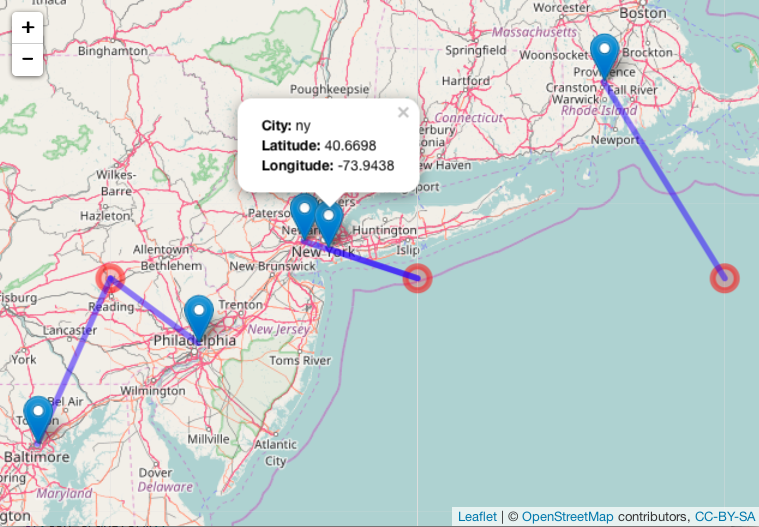
\includegraphics[width = 0.9\textwidth]{ExampleLeaflet}
\end{center}
\caption{Snapshot of an interactive map created using the \code{map\_grid\_leaflet} showing the locations of study cities and their matching climate model grid points for the BCC climate model example data included with \pkg{futureheatwaves}. The lines on the map connect each climate model grid point to the study location(s) for which that grid point was used. The interactive maps include pop-ups with city identifiers; one is shown open in this snapshot as an example. From this map, you can see that the climate model grid point closest to New York City for this climate model is over the Atlantic Ocean.}
\label{fig:gridmap}
\end{figure}

Finally, it can be useful to explore the location of the climate model
grid point used to pull climate model output for each study location
with a given climate model. Therefore, the package has a function called
\texttt{map\_grid\_leaflet} that plots the locations of grid points used
for each location from each climate model. This function is built using
the htmlWidget \CRANpkg{leaflet} package \citep{leaflet}. The following
code illustrates the use of this function with the example data to
create Figure \ref{fig:gridmap}, which plots the grid points used in the
example data from the BCC climate model in the example data:

\begin{Schunk}
\begin{Sinput}
out <- system.file("extdata/example_results", package = "futureheatwaves")
map_grid_leaflet(plot_model = "bcc1", out = out)
\end{Sinput}
\end{Schunk}

\noindent This interactive map can be panned and zoomed to explore the
locations of climate model grid points used to represent each study
location. This mapping function works for study locations worldwide.

\subsection{Extensions}\label{extensions}

While this package was created to be used for research on extreme events
in climate change projections, it can be used more broadly. For example,
there are other episodes like wildfires and air pollution where it may
be interesting to identify extended periods of high exposures in
projection time series. The \pkg{futureheatwaves} package is not
exclusive to CMIP5 model output data, and so could be applied to gridded
air pollution model output to explore these exposures.

\section{Future directions for working with climate model output in
R}\label{future-directions-for-working-with-climate-model-output-in-r}

Research that assesses the potential impacts of climate change is
critical in informing current policy choices, and R is an important tool
for many researchers performing such assessments. While the
\texttt{futureheatwaves} package described here takes steps to
facilitate the assessment of impacts related to sustained, multi-day
events, a number of challenges remain in working with climate model
output data in R, and future R software development offers the potential
to further address the challenges of working with this data.

One important step in future development of R software to work with
climate model output could be the development of R wrappers for some of
the existing command line tools available through the Climate Data
Operators (CDO) software \citep{schulzweida2006cdo}. Libraries already
exist for Python and Ruby that allow the functionality of CDO tools to
be used within these scripting languages (available from the Max Planck
Institute at
\url{https://code.zmaw.de/projects/cdo/wiki/Cdo%7Brbpy%7D}). While one R
package (\CRANpkg{ncdf4.helpers}; \citet{ncdf.4helpers}) already
provides R wrappers for a few CDO operators, such functionality could be
extended through future R software to capture more of the full
functionality of the CDO toolkit.

Another important path for development could be through approaches that
allow researchers to take advantage of the statistical tools offered by
R while maintaining large climate model output files in a netCDF format.
For example, Goncalves and coauthors recently described a ``round table"
approach of connecting as-needed data access from netCDF climate data
files through to functionality available in R and CDO through the
intermediary of a MonetDB database system \citep{goncalves2015round}.

In other topical areas, R programmers are also improving the efficiency
of working with data in large netCDF files through approaches that work
with the data on-disc {[}?{]}. For example, the recent Bioconductor
package \pkg{openCyto} {[}?{]} allows scientists to work with the large
files generated by flow cytometry that characterize cell populations in
a sample. Similar approaches have been taken in metabolomics (e.g.,
{[}packages{]}) and other 'omics fields. The developers of future R
packages to work with climate model output may find it useful to borrow
ideas from these fields to create solutions with improved memory
management {[}?{]} for large climate output files.

\section{Acknowledgements}\label{acknowledgements}

This work was supported by grants from the National Institute of
Environmental Health Sciences (R00ES022631), the National Science
Foundation (1331399), and the Colorado State University Vice President
for Research. Thank you to early testers of the package: Julia
Bromberek, Wande Benka-Coker, Josh Ferreri, Ryan Gan, Molly Gutilla,
Mike Lyons, Casey Quinn, Rachel Severson, and Meilin Yan.

\bibliography{Anderson}

\address{%
G. Brooke Anderson\\
Colorado State University\\
Department of Environmental \& Radiological Health Sciences\\ 1681 Campus Delivery\\ Fort Collins, Colorado 80523\\
}
\href{mailto:brooke.anderson@colostate.edu}{\nolinkurl{brooke.anderson@colostate.edu}}

\address{%
Colin Eason\\
Colorado State University\\
Department of Computer Science\\ 1873 Campus Delivery\\ Fort Collins, Colorado 80523\\
}
\href{mailto:aimesce@gmail.com}{\nolinkurl{aimesce@gmail.com}}

\address{%
Elizabeth A. Barnes\\
Colorado State University\\
Department of Atmospheric Science\\ 1371 Campus Delivery\\ Fort Collins, CO 80523\\
}
\href{mailto:eabarnes@atmos.colostate.edu}{\nolinkurl{eabarnes@atmos.colostate.edu}}

